まず、$\mathrm C_{70}$分子が、電子などの微視的実体に比べて、どれほど重いかを実感しよう。
\begin{figure}[htbp]\centering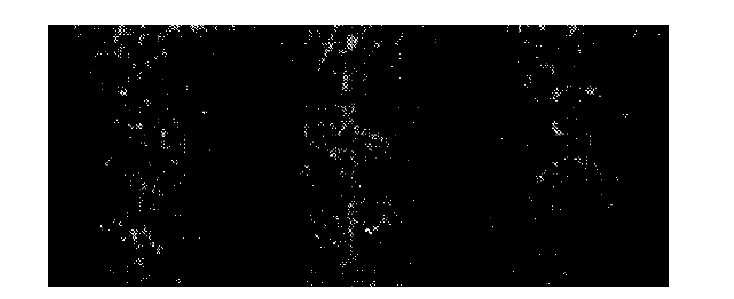
\includegraphics[width=.85\linewidth]{figures/ch06_fig06.pdf}
\caption{Tonomuraたち\cite{ref261}の二重スリット実験で得られた、単一電子の干渉模様。許可を得て\cite{ref261}から転載。Copyright 1989 American Institute of Physics.}
\end{figure}
% 原文 p.260
\hypertarget{srcpage:260}{}\label{srcpage:260}
各炭素原子は6個の陽子、6個の中性子、6個の電子を含むので、$\mathrm C_{70}$分子は合計1000個以上の微視的構成要素からなる。各分子は、高度に励起された内部回転・振動自由度を非常に多数持つ。このため、個々の分子に有限の温度を割り当てることができる。また、分子からの熱放射、すなわち光子の放出も観測できる\cite{ref267}。したがって、$\mathrm C_{70}$分子は、明らかに「粒子」の分類に入るように見える。
\begin{figure}[htbp]\centering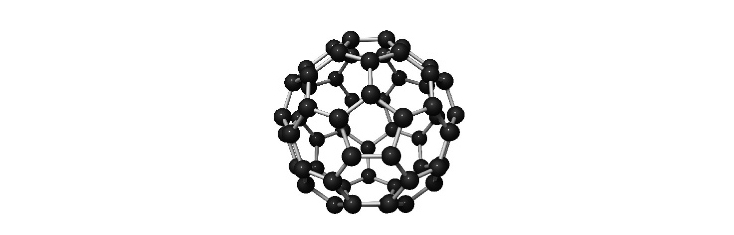
\includegraphics[width=.65\linewidth]{figures/ch06_fig07.pdf}
\caption{Arndtら\cite{ref263}の最初の物質波干渉実験で用いられた、$\mathrm C_{60}$分子の模式図。60個の炭素原子が、直径約1nmのバッキーボール形に並んでいる。}
\end{figure}

このような重い分子の干渉効果を観測するのは、なぜ難しいのだろうか。関係する量は、物質のde Broglie波長$\lambda=h/(mv)$であり、$m$、$v$はそれぞれ粒子の質量と速度である。したがって、粒子が重く速いほど、波長は短い。二重スリット型の実験で粒子の干渉を観測するには、スリット間隔、まして各スリットの幅が、波長程度でなければならない。実験の$\mathrm C_{70}$分子の典型的速度、約$100\,\mathrm{m/s}$では、de Broglie波長はわずか数pmである。このような狭いスリットを、これほど狭い間隔で作ることが不可能なのは、容易に想像できるだろう。

この困難をどう克服できるだろうか。Zeilingerのグループは、いわゆるTalbot--Lau効果に基づく、巧みな仕掛けで解決する。その基本原理は次のとおりである（図6.8参照）。平面波$f(z)=e^{2\pi iz/\lambda}$が、$+z$方向に進むとする。この入射波に直角に、平行なスリットの列からなる格子を置く。隣り合うスリットの間隔を$d$とする。このとき、格子の後方の距離
\begin{equation}L_\lambda=\frac{d^2}{\lambda}\tag{6.29}\end{equation}
の整数倍のところで、波の形が実際に格子模様と等しくなることを示せる。ここでは導かないが、短い導出は\cite{ref268}を参照されたい。言い換えれば、格子の後方$nL_\lambda$、$n=1,2,\ldots$の距離にスクリーンを置き、光で実験すると、
% 原文 p.261
\hypertarget{srcpage:261}{}\label{srcpage:261}
間隔$d$の明暗の帯が現れ、格子自体の像を作る。このTalbot--Lau効果は、真の干渉現象である。したがって、物質粒子で同じ実験を行い、「Talbot長」$L_\lambda$の整数倍のところに、格子模様と等しい密度模様を観測すれば、粒子の波動性を示したことになる。ただし、原理的には、格子が単に光線を遮る、いわゆるMoiré効果でも縞が生じる。しかしMoiré模様は波長$\lambda$に依存しない。ゆえに、本当にTalbot--Lau効果かを確かめるには、$\lambda$を変えながら模様の変化を観測すればよい。物質波の場合、$\lambda=h/(mv)$なので、粒子の平均速度$v$を変えることで実現する。
\begin{figure}[htbp]\centering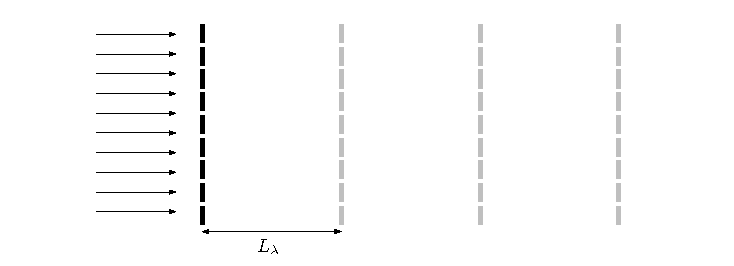
\includegraphics[width=.85\linewidth]{figures/ch06_fig08.pdf}
\caption{Talbot--Lau効果。左の格子を通る平面波は、格子から距離$nL_\lambda$、$n=1,2,\ldots$のところに、格子の像を作る。}
\end{figure}

簡単な評価から、$\mathrm C_{70}$分子の干渉効果を検出するTalbot--Lau法の利点を、直ちに納得できる。Zeilingerのグループの実験では、格子間隔$d$は約$1\,\mu\mathrm m$、分子波長は数pmである。したがって$L_\lambda\sim(10^{-6}\,\mathrm m)^2/(10^{-12}\,\mathrm m)=1\,\mathrm m$となり、干渉模様を観測するには、格子の後方の巨視的距離$L_\lambda$に、「スクリーン」、すなわち粒子検出器を置くだけでよい。実際の実験距離は$L_\lambda=38\,\mathrm{cm}$である。そこで分子速度を変えたとき、特徴的な波長依存性を示す、周期$d$の粒子密度変化を測定すれば、分子の波動性を確認したことになる。

実験配置を図6.9に示す。$\mathrm C_{70}$分子は源から放出され、同一の自立型金格子を三枚通る。各格子は、周期$d=990\,\mathrm{nm}$のスリットを1000本程度含む。最初の格子は、回折模様が観測できるよう、ビームへ一定のコヒーレンスを与える。中央の格子が、実際の回折格子として働く。最後に第三の格子を、回折格子の後方、Talbot長$L_\lambda$の距離に置く。
% 原文 p.262
\hypertarget{srcpage:262}{}\label{srcpage:262}
これは、分子が実際に波動性を持つなら、第三格子の位置で回折格子自体の像となる、干渉模様が得られることを意味する。すなわち、分子密度は$x$方向に周期的な極大と極小を持ち、ピークはスリット間隔$d$だけ離れる。第三格子は、この分子密度模様を走査するマスクである。干渉模様があれば、格子を$x$方向へ動かすと、その後方で記録される分子数が最大値と最小値の間で変動する。したがって、第三格子後方の分子数を、格子の$x$位置の関数として数えることで、この変動を容易に測れる。
\begin{figure}[htbp]\centering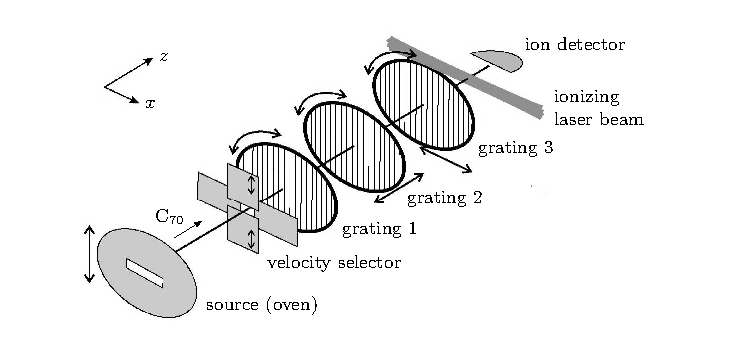
\includegraphics[width=.85\linewidth]{figures/ch06_fig09.pdf}
\caption{Zeilingerのグループの実験\cite{ref264,ref265,ref266,ref267}で、$\mathrm C_{70}$分子の物質波干渉を観測する配置。許可を得て\cite{ref264}の図を改作。Copyright 2002 by the American Physical Society.}
\end{figure}

装置を通る分子の平均速度は、分子源の位置を変え、自由飛行放物線を描くビームの異なる部分を、固定高さの制限器で選ぶことで、約90から$220\,\mathrm{m/s}$の間で調整できる。これらは、de Broglie波長2から6pmに対応する。分子と他粒子の衝突を最小にするため、装置全体は真空槽に収められている。

\subsubsectionlink{重い分子の波動性を確かめる}
典型的な実験一回の結果を図6.10に示す。横軸は走査マスクの$x$軸方向の位置（図6.9参照）、縦軸は各位置における格子後方の分子密度である。$\mathrm C_{70}$分子密度の振動が明瞭に見え、空間的コヒーレンスと干渉効果の存在を確認できる。
% 原文 p.263
\hypertarget{srcpage:263}{}\label{srcpage:263}
分子速度を変え、Talbot--Lau理論に一致する密度模様の変化を観測することで、この模様が実際にTalbot--Lau効果によることも明示的に確認された。
\begin{figure}[htbp]\centering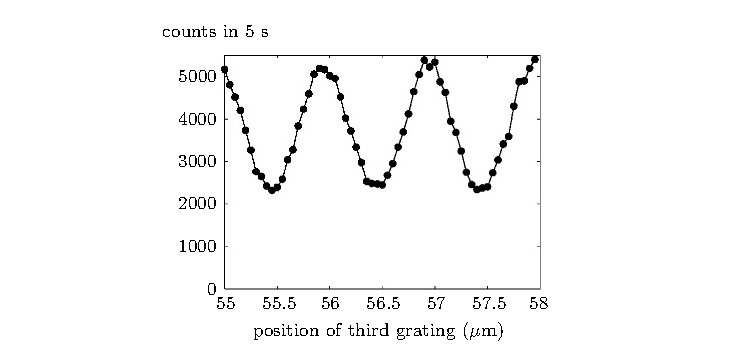
\includegraphics[width=.82\linewidth]{figures/ch06_fig10.pdf}
\caption{Zeilingerのグループの実験で観測された、$\mathrm C_{70}$分子の干渉縞。実線は理論予測に基づいて当てはめた正弦曲線である。許可を得て\cite{ref264}の図を改作。Copyright 2002 by the American Physical Society.}
\end{figure}

また、干渉効果は厳密な一粒子効果であり、異なる分子間の干渉によるものではない。理由は二つある。第一に、粒子間干渉には、相互作用する分子が同じ状態である必要がある。しかし、各$\mathrm C_{70}$分子は非常に多数の内部自由度を持つため、その可能性は実効的にゼロである。第二に、二分子間の距離は、いかなる分子間力の範囲よりもはるかに大きく、したがって、本質的に、どの瞬間にも装置を通っているのは単一分子だけである。

\subsubsectionlink{経路情報とデコヒーレンス}
それでは、本章の主要主題である、デコヒーレンスの実験観測へ移ろう。$\mathrm C_{70}$干渉実験では、デコヒーレンスは主として、分子と背景気体の分子の衝突による。真空は完全ではないので、背景気体は装置内にある程度常に存在する。このような衝突デコヒーレンスは第3章で詳しく述べ、自然界に普遍的にある源であることを示した。しかし、本章冒頭で述べたように、中間的尺度や巨視的物体では、それが通常あまりに速く、その漸進的作用を観測することは実効的に不可能である。
% 原文 p.264
\hypertarget{srcpage:264}{}\label{srcpage:264}
ここに、$\mathrm C_{70}$干渉実験の主要な利点がある。背景気体密度を変えることで、衝突デコヒーレンスの量を精密に調整できる。図6.11は、Lucia Hackermüllerら\cite{ref268}が報告した、背景気体の二つの圧力、すなわち密度で実験的に測定された干渉模様である（\cite{ref265}も参照）。左の図では、干渉縞が明瞭に見える。背景気体の圧力を高めると、縞が目立たなくなる（右）。圧力$p$における干渉模様の可視度$V(p)$を、その最大振幅$c_{\max}(p)$と最小振幅$c_{\min}(p)$の相対差として定量化しよう。
\begin{equation}V(p)=\frac{c_{\max}(p)-c_{\min}(p)}{c_{\max}(p)+c_{\min}(p)}.\tag{6.30}\end{equation}
デコヒーレンスも他の実験的不完全さもない理想的場合には、$c_{\min}=0$で、完全な可視度を得る。完全にデコヒーレンスした場合、干渉模様は観測できず、$c_{\max}=c_{\min}$となるので、可視度はゼロである。

気体圧力$p$に対する可視度(6.30)の変化の実験データ\cite{ref265,ref268}を、図6.12に示す。可視度は$p$とともに指数関数的に低下する。縦軸が対数目盛であることに注意されたい。この指数減衰は、理論計算\cite{ref160,ref269}と見事に一致する。
\begin{figure}[htbp]\centering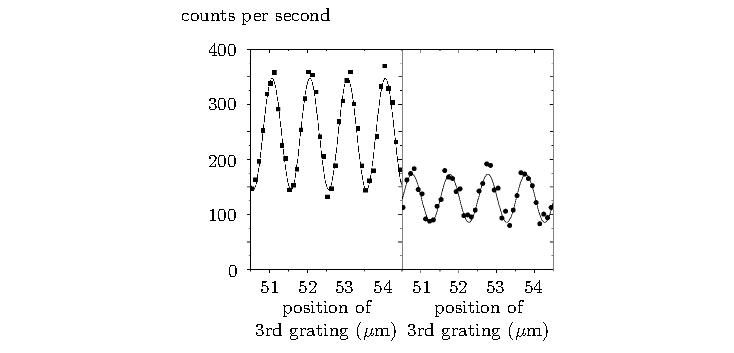
\includegraphics[width=.86\linewidth]{figures/ch06_fig11.pdf}
\caption{Zeilingerのグループの実験\cite{ref268}で観測された、背景気体分子との衝突が誘起するデコヒーレンスによる、$\mathrm C_{70}$分子干渉の減少。左から右へ気体圧力を高めると、干渉縞の可視度が低下する。Springer Science and Business Mediaのご厚意により、許可を得て\cite{ref268}の図を改作。}
\end{figure}
% 原文 p.265
\hypertarget{srcpage:265}{}\label{srcpage:265}
\begin{figure}[htbp]\centering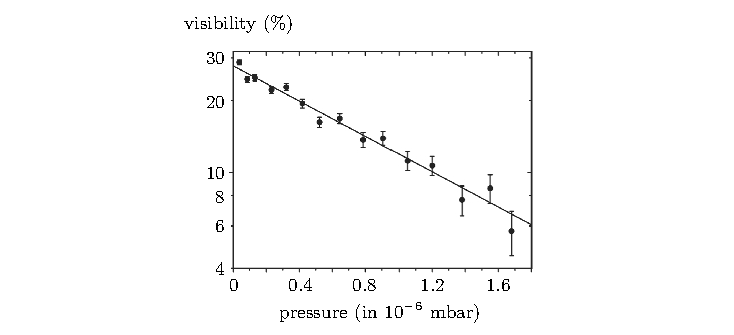
\includegraphics[width=.82\linewidth]{figures/ch06_fig12.pdf}
\caption{Zeilingerのグループ\cite{ref268}が報告した、背景気体圧力への干渉模様の可視度(6.30)の依存性。測定値（円）は、圧力に対する指数減衰を記述する理論予測（実線）によく一致する。Springer Science and Business Mediaのご厚意により、許可を得て\cite{ref268}の図を改作。}
\end{figure}
したがって、これらの実験は、干渉の観測に必要な量子コヒーレンスを、環境との相互作用が徐々に非局在化する様子を、印象的かつ直接に示す。この過程は完全に制御されている。たとえば背景気体の密度を変え、環境が得る経路情報量を変化させれば、デコヒーレンスの量、したがって量子的特徴の喪失を、精密に調整できる。こうして、量子・古典境界を滑らかに行き来して探索でき、観測が理論予測と極めてよく一致することが分かる。

\subsubsectionlink{熱放射の放出によるデコヒーレンス}
巨視的物体の最も重要なデコヒーレンス機構は何だろうか。これまで見たように、光子や空気分子など、他粒子との衝突は確かに普遍的にあり、決定的な役割を果たす。しかし、この長さ尺度でのもう一つの基本的な源は、熱放射の放出である。どの「大きな」物体も、多数の内部自由度へエネルギーを蓄えられる。巨視的物体は、本質的に絶えず光子を吸収し放出する。各放出光子は、物体の経路の情報を運び去り、位置基底でのデコヒーレンス、したがって物体の空間的局在化を生じさせる。

巨視的物体では、熱放射の放出は通常、空間的干渉効果を観測する可能性を完全に閉ざすほど強い。興味深いことに、以下で見るように、$\mathrm C_{70}$分子は、熱的デコヒーレンスに関して微視的領域と巨視的領域の境界を、ちょうどまたいでいる。
% 原文 p.266
\hypertarget{srcpage:266}{}\label{srcpage:266}
可視の干渉模様を生じさせるほど小さい一方、十分複雑であるため、数千Kまで加熱すると、熱的デコヒーレンスによって干渉模様が完全に消える。したがって、これらの分子は、熱的デコヒーレンス効果を明示的に観測するのに理想的である。装置を通過する前に徐々に加熱し、分子温度の関数として干渉縞の可視度の減衰を記録すればよい。

この考えは、Zeilingerのグループが行い、Hackermüllerら\cite{ref267}が2004年に報告した、注目すべき実験で実現された。格子を通る前に、$\mathrm C_{70}$分子は、レーザービームによって、源での約900Kから約3000Kまで加熱された。四つのレーザー出力、したがって分子平均温度について観測された干渉模様を、図6.13に示す。

予想どおり、分子からの熱放射のため、レーザー出力とともに可視度が低下する。さまざまな加熱出力での一連の実験結果を図6.14に示す。実験データは、理論計算\cite{ref267}の予測によく一致する。
\begin{figure}[htbp]\centering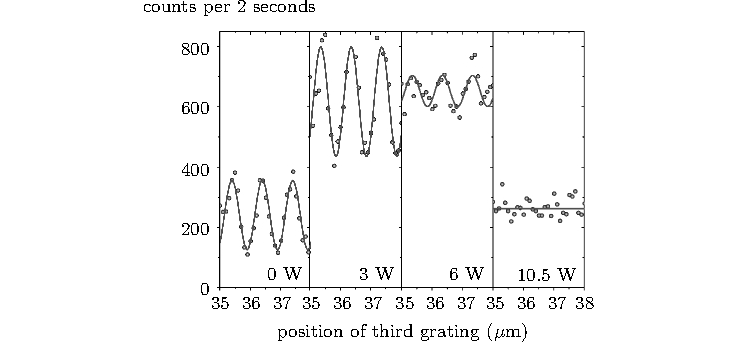
\includegraphics[width=.96\linewidth]{figures/ch06_fig13.pdf}
\caption{Hackermüllerら\cite{ref267}の実験で測定された、異なるレーザー加熱出力、したがって異なる分子平均温度における、$\mathrm C_{70}$分子の干渉模様。平均温度が上がるほど可視度が低下する。異なる加熱出力で全体の平均計数率が変わるのは、分子エネルギーによるイオン計数検出器の効率の変化と、加熱段階での電離・破砕効果による。Macmillan Publishers Ltdの許可を得て\cite{ref267}から転載：Nature, copyright 2004.}
\end{figure}
% 原文 p.267
\hypertarget{srcpage:267}{}\label{srcpage:267}
\begin{figure}[htbp]\centering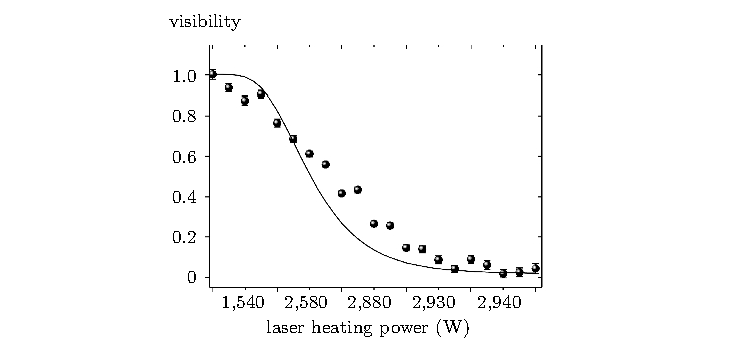
\includegraphics[width=.85\linewidth]{figures/ch06_fig14.pdf}
\caption{Hackermüllerら\cite{ref267}の実験における、レーザー加熱出力と平均分子温度の関数としての、$\mathrm C_{70}$干渉模様の可視度の減衰。円は実験データを表し、実線の理論予測によく一致する。Macmillan Publishers Ltdの許可を得て\cite{ref267}から転載：Nature, copyright 2004.}
\end{figure}
さらに詳しい実験の理論解析は、\cite{ref270,ref271}にある。

結果は、$\mathrm C_{70}$分子が約1000K以下なら、熱的デコヒーレンスは、干渉模様を観測できるほど弱いことを示す。約2000K以上では可視度を有意に低下させ、約3000Kで干渉模様は完全に消える。

これは次のように説明できる。放出光子が、$\mathrm C_{70}$分子の経路を分解できるだけの経路情報を伝えるには、その波長は、分子の異なる経路の隔たり、すなわち回折格子の異なるスリットの通過に対応する波束の極大間隔と、同程度でなければならない。この隔たりはスリット自体の間隔$d\approx1\,\mu\mathrm m$程度なので、熱的デコヒーレンスには、波長$\lambda\lesssim1\,\mu\mathrm m$の光子放出が必要である。分子がこの波長の光子を放出する有意な確率が現れるのは、2000Kを超える温度になってからだと分かる。約3000Kでは、典型的に、そのような光子を数個放出する。これが、干渉模様を完全に破壊するのに十分な経路情報を、環境へ移す。

\subsubsectionlink{バッキーボールを超えて}
$\mathrm C_{70}$分子の一粒子干渉縞が実験で観測された以上、自然な次の段階は、ますます大きな分子で、そのような量子効果を示すことである。
% 原文 p.268
\hypertarget{srcpage:268}{}\label{srcpage:268}
実際、Zeilingerのグループは、Hackermüllerらが2002年に報告した実験\cite{ref266}で、すでに次の一歩を踏み出した。$\mathrm C_{70}$用と同様の配置で、さらに重いフッ素化フラーレン$\mathrm C_{60}\mathrm F_{48}$（質量$m=1632\,\mathrm{amu}$、108原子）と、生体分子テトラフェニルポルフィリン$\mathrm C_{44}\mathrm H_{30}\mathrm N_4$（質量$m=614\,\mathrm{amu}$、幅2nm以上）の干渉模様が観測された。分子構造を図6.15、得られた干渉模様を図6.16に示す。これらの比較的重く複雑な分子でも、明確な干渉縞が観測され、可視度は理論予測によく一致した。
\begin{figure}[htbp]\centering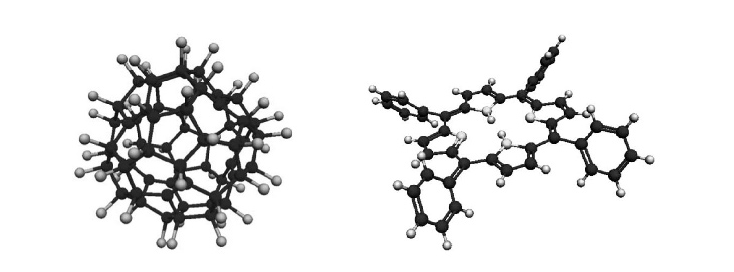
\includegraphics[width=.9\linewidth]{figures/ch06_fig15.pdf}
\caption{Hackermüllerら\cite{ref266}の干渉実験に用いられた、$\mathrm C_{60}\mathrm F_{48}$分子（左）と、生体分子テトラフェニルポルフィリン$\mathrm C_{44}\mathrm H_{30}\mathrm N_4$（右）の三次元構造。許可を得て\cite{ref266}から転載。Copyright 2003 by the American Physical Society.}
\end{figure}
\begin{figure}[htbp]\centering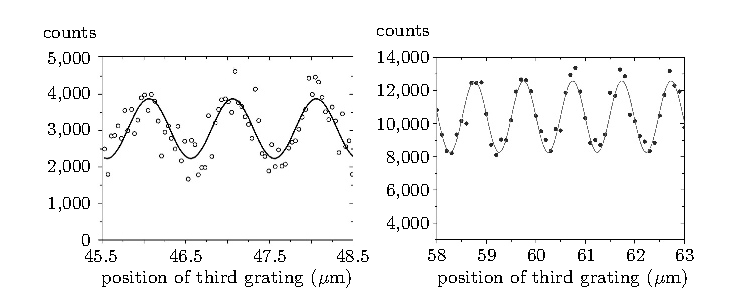
\includegraphics[width=.96\linewidth]{figures/ch06_fig16.pdf}
\caption{Hackermüllerら\cite{ref266}の実験で観測された、$\mathrm C_{60}\mathrm F_{48}$分子（左）と、生体分子テトラフェニルポルフィリン$\mathrm C_{44}\mathrm H_{30}\mathrm N_4$（右）の干渉縞。実線は当てはめた正弦曲線。許可を得て\cite{ref266}の図を改作。Copyright 2003 by the American Physical Society.}
\end{figure}

% 原文 p.269
\hypertarget{srcpage:269}{}\label{srcpage:269}
さらに大きい粒子、たとえばタンパク質やウイルスなどの生体分子\cite{ref268,ref272}、炭素質エアロゾル\cite{ref271}を使う干渉実験の実現可能性も、推測できる。そのような実験は、主に三つの要因で制限される。
\begin{enumerate}
\item 衝突デコヒーレンス。これらの分子の干渉縞を観測するには、装置内の真空が非常によくなければならない。背景気体密度の関数として干渉縞の可視度を記述するデコヒーレンス模型を使い、ライノウイルスの大きさに至るまでの、いくつかの生体分子について、干渉の観測に必要な真空の質が評価された\cite{ref268,ref272}（図6.17参照）。この評価は、現在の約3倍である、格子間隔1mの長いTalbot--Lau干渉計を使えることを仮定するが、これはまだ実験的に実現されていない。この設計なら、必要な低い背景気体密度は、現在の技術で達成できる範囲にある\cite{ref265,ref268}。
\item 熱的デコヒーレンス。大きな尺度では、これがますます重要になる。たとえば、Talbot--Lau干渉計とは異なる単純な二重スリット配置では、小さなウイルス（質量$5\times10^7\,\mathrm{amu}$）が、十分な可視度の干渉模様を示すには、約40Kまで冷却する必要があると評価された\cite{ref271}。そのような「冷たいウイルス」のビームを実験室で作るのは、明らかにかなり難しい。ゆえに、$\mathrm C_{70}$より大きい物体では、
% 原文 p.270
\hypertarget{srcpage:270}{}\label{srcpage:270}
衝突デコヒーレンスよりも、熱的デコヒーレンスの影響を弱める方が、実験的にははるかに難しくなるかもしれない\cite{ref271}。
\item 慣性力と振動による位相緩和。それ自体はデコヒーレンス効果ではないが、地球の質量と回転、回折格子の振動によって誘起される、重力的、回転的、音響的擾乱の雑音も、可視度へ影響する\cite{ref273}。これらは干渉縞の観測可能性を強く制限し得るので、実験者は、ここで述べたTalbot--Lau配置で、これらの雑音源を最小にすることに大きな注意を払っている。それでも、図6.17の粒子では、振動雑音が干渉観測の大きな障害になると予想される\cite{ref273}。現在利用できる配置では、その雑音は、衝突・熱的デコヒーレンス以上に、可視度を低下させる可能性が高い。
\end{enumerate}
\begin{figure}[htbp]\centering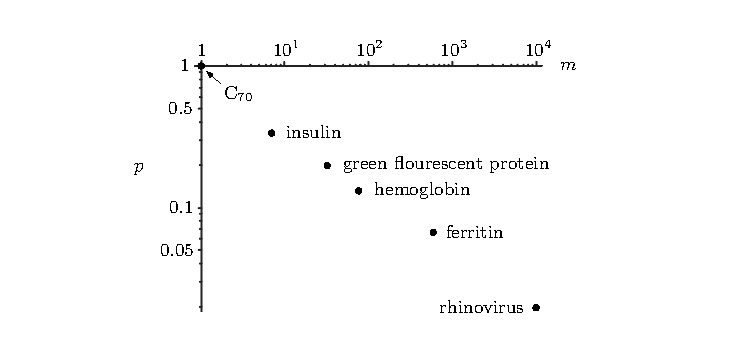
\includegraphics[width=.85\linewidth]{figures/ch06_fig17.pdf}
\caption{長いTalbot--Lau干渉計で、いくつかの生体分子の干渉縞を観測できる、背景気体の最大圧力$p$の評価。横軸は$\mathrm C_{70}$分子の質量を基準とする分子量$m$。縦軸の圧力は、$\mathrm C_{70}$の干渉観測に必要な圧力で規格化している。Hackermüllerら\cite{ref268}のデータから作図。}
\end{figure}

しかし、念頭に置くべき重要な点は、理論的デコヒーレンス模型を用い、干渉効果を観測する条件を精密に指定し定量化できることである。Copenhagen解釈が仮定するような、曖昧に定義された、量子領域と古典領域の基本的区分という仮定に、もはやとどまる必要はない。代わりに、対象分子を環境と相互作用する開いた量子系として扱うことで、干渉を観測するために何をすべきか、特定の実験設定でなぜ干渉縞が観測できないかを、理解できる。

$\mathrm C_{70}$分子は、周囲の粒子との衝突と熱放射の放出によるデコヒーレンスの、漸進的作用の観測を可能にする、ちょうどよい感受性を持つ。したがって、系を古典領域へ導くデコヒーレンスの、直接的で制御可能な影響を示す、これ以上分かりやすく直観的な実験を想像することは難しい。将来の干渉実験は、その限界をさらに巨視的領域へ押し進めると期待され、この分野の研究の進展を追うのは楽しみである。
